\documentclass{article}
 

 
\usepackage[margin=1in]{geometry} 
\usepackage{amsmath,amsthm,amssymb}
 \usepackage{graphicx}
 \usepackage{enumerate}
 \usepackage{color}
 \usepackage{hyperref}
 
 \hypersetup{urlcolor=cyan}
 
\newcommand{\N}{\mathbb{N}}
\newcommand{\Z}{\mathbb{Z}}

\newcommand\numberthis{\addtocounter{equation}{1}\tag{\theequation}}

\def\R{\mathbb{R}}
\def\Zp{\mathbb{Z}^+}

\def\a{\alpha}
\def\b{\beta}
\def\c{\gamma}

 
\begin{document}
 
% --------------------------------------------------------------
%                         Start here
% --------------------------------------------------------------
 
 
%%%%%%%%%%%%%%%%%%%%%%%%%%%%%%%%%
% TITLE PAGE
%%%%%%%%%%%%%%%%%%%%%%%%%%%%%%%%% 
\title{
    \textmd{\Huge{Midterm B2}}\\
    \textmd{\huge{Section 2}}
}


\maketitle

Consider the set of points $(-2, 3)$, $(1, 2)$ and $(2, 3)$ and the interpolating polynomial $f(x)$, which is a $2^\text{nd}$ degree polynomial that passes through those points. \\

\textbf{Problem 1} [15pt]: Write down $f(x)$ as a Lagrangian polynomial.

Before anything, I do a quick \textit{qualitative} sketch to see what's going on. \hspace*{3cm}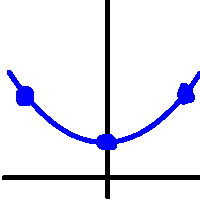
\includegraphics[scale=0.5]{thumbSketch}\\

Since we're told that $f$ is a $2^\text{nd}$ degree polynomial, we know that $f$ is either a parabola, a line, or a point. It's clear from my sketch that it has to be a parabola opening upwards. If that's the case, then for $f(x) = \a x^2 + \b x + \c$, we must have $\a$ strictly greater than $0$. It turns out that this quick analysis will not help us too much for \textit{this} problem, but it never hurts to start with an idea of what's going on. That way, if I end up with something like $\a = -2$ in the end, I'll know that I messed up somewhere. \\

Now that we got that out of the way, let's think of how we write a Lagrangian polynomial when given 3 points. For points $(x_1, y_1)$, $(x_2, y_2)$ and $(x_3, y_3)$, we have the formula \\

\[
f(x)  = y_1 \frac{(x - x_2)(x - x_3)}{(x_1 - x_2)(x_1 - x_3)} + y_2 \frac{(x - x_1)(x - x_3)}{(x_2 - x_1)(x_2 - x_3)} + y_3 \frac{(x - x_1)(x - x_2)}{(x_3 - x_1)(x_3 - x_2)} \numberthis
\] \\

Notice how nicely the "$ - \, x_i $" terms look stacked on top of each other like that. In the first fraction we have $x_2$ right over $x_2$ and the $x_3$ over the $x_3$. The situation is similar for the other two fractions. Also notice that $f$ is a function of $x$. There are two $x$'s in each numerator. Some people made the mistake of substituting point values in for the $x$'s in (1). That's not good. Suppose we didn't have any $x$'s in our expression. Then (1) would just be a sum of constants, giving you some scalar $C$.  You'd have $f(x) = C$, and there's \textit{no way} that $f(x)$ could go through the 3 points I drew horribly up top. \\

Also, notice that our sketch implies that if we multiply out (1) to get some expression $f(x) = \a x^2 + \b x + \c$, then $\a$ better be nonzero and positive. This \textbf{can not} happen if we don't have two $x$'s in the numerators. One other thing to note is that we're given 3 points, and we have 3 expressions in (1). Look at where the $y_1$ and $x_1$'s appear in the first fraction. Look at how similar that is to $y_2$ and the $x_2$'s in the second fraction. \\

Let's take a second to think about how we could generalize (1) a little. That is, suppose we were given four points, $(x_1, y_1)$, $(x_2, y_2)$, $(x_3, y_3)$, and $(x_4, y_4)$ and we want a corresponding Lagrangian polynomial $g(x)$. Without knowing "the formula" for a $4^\text{th}$ order Lagrangian polynomial, I'm just going to set it up the way (1) is set up: \\

\[
g(x)  = y_1 \frac{(x - x_2)(x - x_3)}{(x_1 - x_2)(x_1 - x_3)} + y_2 \frac{(x - x_1)(x - x_3)}{(x_2 - x_1)(x_2 - x_3)} + y_3 \frac{(x - x_1)(x - x_2)}{(x_3 - x_1)(x_3 - x_2)}  + y_4 \frac{(x - ?)(x - ?)}{(x_4 - ?)(x_4 - ?)} 
\] \\

If three points determines a $2^\text{nd}$ order polynomial, it makes sense that four points determine a $3^\text{rd}$ order polynomial. Then we'll need something like this $(x - a)(x- b)(x-c)$ in each numerator. \\

\[
g(x)  = y_1 \frac{(x - x_2)(x - x_3)(x - ?)}{(x_1 - x_2)(x_1 - x_3)} + y_2 \frac{(x - x_1)(x - x_3)(x - ?)}{(x_2 - x_1)(x_2 - x_3)} + y_3 \frac{(x - x_1)(x - x_2)(x - ?)}{(x_3 - x_1)(x_3 - x_2)}  + y_4 \frac{(x - ?)(x - ?)(x - ?)}{(x_4 - ?)(x_4 - ?)} 
\] \\

By analogy, I'm assuming there must also be extra terms in the denominator. Note that the first $x_i$ in each denominator agrees with the $y_i$ in (1). We'll do the same thing here.\\

\[
g(x)  = y_1 \frac{(x - x_2)(x - x_3)(x - ?)}{(x_1 - x_2)(x_1 - x_3)(x_1 - ?)} + y_2 \frac{(x - x_1)(x - x_3)(x - ?)}{(x_2 - x_1)(x_2 - x_3)(x_2 - ?)} + y_3 \frac{(x - x_1)(x - x_2)(x - ?)}{(x_3 - x_1)(x_3 - x_2)(x_3 - ?)}  + y_4 \frac{(x - ?)(x - ?)(x - ?)}{(x_4 - ?)(x_4 - ?)(x_4 - ?)} 
\] \\

Now we just fill in the $?$'s in the obvious way, taking care not to \textit{ever} divide by zero \dots \textit{ever}.

\begin{align*}
g(x)  = &y_1 \frac{(x - x_2)(x - x_3)(x - x_4)}{(x_1 - x_2)(x_1 - x_3)(x_1 - x_4)} + y_2 \frac{(x - x_1)(x - x_3)(x - x_4)}{(x_2 - x_1)(x_2 - x_3)(x_2 - x_4)} +  \\
& y_3 \frac{(x - x_1)(x - x_2)(x - x_4)}{(x_3 - x_1)(x_3 - x_2)(x_3 - x_4)}  + y_4 \frac{(x - x_1)(x - x_2)(x - x_3)}{(x_4 - x_1)(x_4 - x_2)(x_4 - x_3)} 
\end{align*}

And we've just blindly derived the general form of a $4^\text{th}$ order Lagrangian polynomial by reason and analogy alone. My point with this is that if you know the formula for a $1^\text{st}$ order Lagrangian polynomial given two points, then you have the resources to figure out the formula for a $2^\text{nd}$ order Lagrangian polynomial, given 3 points. You just have to be a little creative and notice the patterns. \\

Back to the problem. Technically, you could write this

\[
f(x)  = y_1 \frac{(x - x_2)(x - x_3)}{(x_1 - x_2)(x_1 - x_3)} + y_2 \frac{(x - x_1)(x - x_3)}{(x_2 - x_1)(x_2 - x_3)} + y_3 \frac{(x - x_1)(x - x_2)}{(x_3 - x_1)(x_3 - x_2)} 
\]
\[
\text{where} \quad \begin{pmatrix} x_1 \\ x_2 \\ x_3 \end{pmatrix}  = \begin{pmatrix} -2 \\ 1 \\ 2 \end{pmatrix} \quad \text{and} \quad  \begin{pmatrix} y_1 \\ y_2 \\ y_3 \end{pmatrix}  = \begin{pmatrix} 3 \\ 2 \\ 3 \end{pmatrix} \numberthis
\] \\

{\setlength{\parindent}{0cm}
and it would be a perfectly good answer. I'm surprised nobody tried that. Some people did this}\\

\[
f(x)  = 3 \frac{(x - 1)(x - 2)}{(-2  - 1)(-2  - 2)} + 2 \frac{(x + 2)(x - 2)}{(1 + 2)(1 - 2)} + 3 \frac{(x + 2)(x - 1)}{(2 + 2)(2 - 1)} \numberthis \\
\] \\

{\setlength{\parindent}{0cm}
and I thanked you for it. Most people reduced the denominators like this} \\

\[
f(x)  = 3 \frac{(x - 1)(x - 2)}{12} + 2 \frac{(x + 2)(x - 2)}{-3} + 3 \frac{(x + 2)(x - 1)}{4} \numberthis \\
\] \\

{\setlength{\parindent}{0cm}
or this} \\

\[
f(x)  =  \frac{(x - 1)(x - 2)}{4} -  \frac{2(x + 2)(x - 2)}{3} + \frac{3(x + 2)(x - 1)}{4} \numberthis \\
\] \\

{\setlength{\parindent}{0cm}
and it was only mildly annoying. Of course, if you were really high-speed, you did this} \\

\begin{align*}
f(x)  &=  \frac{(x - 1)(x - 2)}{4} -  \frac{2(x + 2)(x - 2)}{3} + \frac{3(x + 2)(x - 1)}{4} \\
&= \frac{x^2 - 3 x +2}{4} - \frac{2x^2  - 8}{3} + \frac{3 x^2 + 3 x - 6}{4} \\
&= \left( \frac{1}{4} - \frac{2}{3} + \frac{3}{4} \right) x^2 + \left( -\frac{3}{4} + \frac{3}{4} \right) x + \left( \frac{2}{4} + \frac{8}{3} - \frac{6}{4} \right) \numberthis \\
&= \frac{1}{3} x^2 + 0 x + \frac{5}{3} \\
&= \frac{1}{3} x^2 + \frac{5}{3} 
\end{align*}\\

{\setlength{\parindent}{0cm}
and you ended up doing way more work than necessary. However, now we have $f(x)$ in the form $f(x) = \a x^2 + \b x + \c$, where $\a > 0$ just as we expected. At least if you went this far, you can double-check that your result (i.e. $f(x) = x^2 / 3 + 5 / 3$) is consistent with the sketch. }\\

If you (accurately) wrote anything like (2) through (6) above, then you should have been awarded 15 points. If you wrote down the general formula (1), then you more or less solved the problem. I need to know, however, that you know \textit{which} points go into each $x_i$ and $y_i$. I tried to be fair and overlooked \textit{a lot} of algebraic mistakes. Most of these mistakes occurred after people had (correctly) written down (3)! \\

If you're taking an exam and you're working on a problem like this, \textbf{stop once you've reached (3)}. Go work on other problems. If you still feel like cranking out calculations because you're not sure what the grader is looking for, come back to it after you've attempted all the other problems. 

\end{document}











































